
\section{Experimentation}
\label{sec:experimentation}

% \begin{figure*}
%   \begin{center}
%     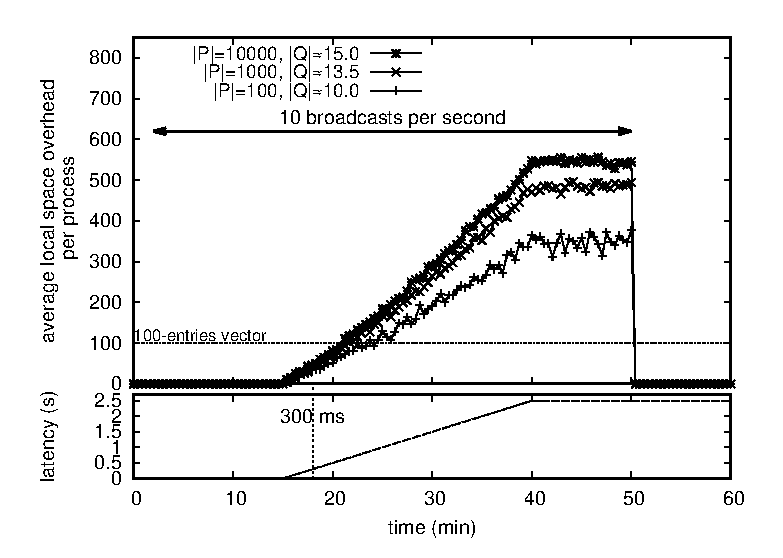
\includegraphics[width=0.65\textwidth]{./img/overhead.eps}
%     \caption{\label{fig:overhead}Local space overhead over time consumed by
%       \RPCBROADCAST to ensure causal order and forbid double delivery in dynamic
%       systems with varying latency.}
%   \end{center}
% \end{figure*}

\begin{figure*}
  \begin{center}
    \begin{subfigure}[t]{0.495\textwidth}
    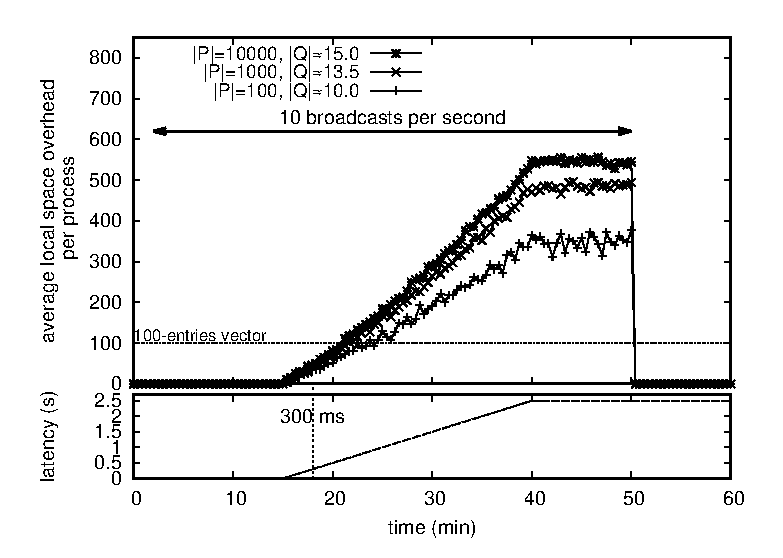
\includegraphics[width=1\textwidth]{./img/overhead.eps}
    \caption{\label{fig:overhead}Local space overhead.}
    \end{subfigure}
    \begin{subfigure}[t]{0.495\textwidth}      
      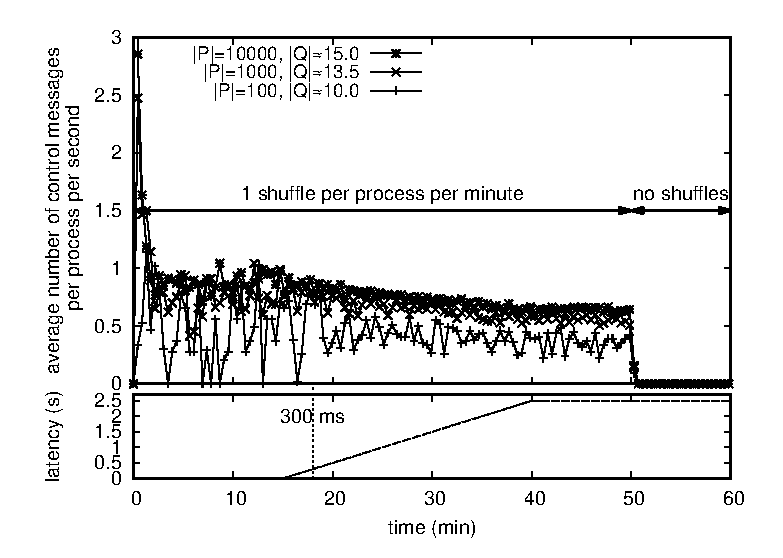
\includegraphics[width=1\textwidth]{./img/controlmessages.eps}
      \caption{\label{fig:controlmessages}Generated traffic overhead (includes
        routing).}
    \end{subfigure}
    \caption{Overhead of \RPCBROADCAST required to ensure causal order and
      forbid multiple delivery in dynamic systems with varying latency.}
  \end{center}
\end{figure*}


\RPCBROADCAST proposes a novel trade-off between speed, memory, and
traffic. Most importantly, its space consumed varies over receipts. In this
section, we evaluate the impact of the actual system on the space consumed and
traffic generated by processes. The experiments run on the \PEERSIM
simulator~\cite{montresor2009peersim} that allows to build large and dynamic
systems. Our implementation is available on the Github platform at
\url{http://github.com/chat-wane/peersim-prcbroadcast}.


% \begin{figure}
%   \begin{center}
%   
\begin{tikzpicture}[scale=0.6]

  \small
  
  \newcommand\X{1.45*\columnwidth/8pt};
  \newcommand\YA{0pt};
  \newcommand\YB{-60pt};


  \draw[->](0*\X, \YA) -- (9*\X, \YA);
  \draw[->](0*\X, \YB) -- (9*\X, \YB);
  
  \draw[fill=white] (0*\X, \YA) node{\textbf{\textup{A}}}
  +(-5pt, -5pt) rectangle +(5pt, 5pt);
  \draw[fill=white] (0*\X, \YB)  node{\textbf{\textup{B}}}
  +(-5pt, -5pt) rectangle +(5pt, 5pt);

  % \draw ( 1*\X, \YA ) node[above]{$\mathcal{A}$};
  % \draw ( 1*\X, \YB ) node[below]{$\mathcal{B}$};

  \draw[->] ( 2*\X, \YA ) -- node[sloped, above]{$\alpha$} (3*\X, \YB);
  % node[below left]{$\mathcal{A}$};

  \draw[decorate,decoration={brace,amplitude=6pt,mirror,raise=4pt}] (3*\X,
  -5+\YB) -- node[anchor=north, yshift=-10pt]{$B_{B\alpha}$}
  (5*\X, -5+\YB);

  % \draw ( 3*\X, \YA ) node[above]{$\mathcal{C}$};

  \draw[->] ( 3*\X, \YB ) -- node[sloped, above]{$\beta$} (4*\X, \YA);
  % node[above left]{$\mathcal{B}$};

  \draw[decorate,decoration={brace,amplitude=6pt,raise=4pt}] (4*\X,
  5+\YA) -- node[anchor=south, yshift=10pt]{$B_{A\beta} \bm{= B_{A\alpha}}$}
  (6*\X, 5+\YA);

  \draw[decorate,thick,decoration={brace,amplitude=6pt,raise=4pt}] (6*\X,
  5+\YA) -- node[anchor=south, yshift=10pt]{$\bm{B_{A\pi}}$}
  (8*\X, 5+\YA);
  
  
  % \draw ( 4*\X, \YB ) node[below]{$\mathcal{D}$};

  \draw[->] ( 4*\X, \YA ) -- node[sloped, above]{$\pi$} (5*\X, \YB);
  % node[below left]{$\mathcal{C}$};

  \draw[decorate,decoration={brace,amplitude=6pt,mirror,raise=4pt}] (5*\X,
  -5+\YB) -- node[anchor=north, yshift=-10pt]{$B_{B\pi} \bm{= B_{B\beta}}$}
  (7*\X, -5+\YB);


  % \draw ( 5*\X, \YA ) node[above]{$\mathcal{E}$};

  \draw[->] ( 5*\X, \YB ) -- node[sloped, above]{$\rho$} (6*\X, \YA);
  % node[above left]{$\mathcal{D}$};
  
  % \draw (6*\X, \YB) node[below]{$\mathcal{F}$};

  \draw[->, dashed] ( 6*\X, \YA ) -- node[sloped, above]{$B_{A\beta}$} (7*\X, \YB);

  \draw[->, dashed, thick] ( 7*\X, \YB ) --
  node[sloped, below]{$\bm{B_{B\beta}}$} (8*\X, \YA);

%  node[below left]{$\mathcal{E}$};


\end{tikzpicture}

%%% Local Variables:
%%% mode: latex
%%% TeX-master: "../paper"
%%% End:

%   \caption{\label{fig:bibroadcast}\RPCBROADCAST ensures the safety of bidirectional links
%     at marginal cost. Process~A maintains an additional buffer. Process~B transmits its
%     second buffer.}
%   \end{center}
% \end{figure}

\noindent \textbf{Objective:} To confirm that local space complexity
depends on in-views and message receipts.

\noindent \textbf{Description:} We measure the average size of buffers and
arrays of expected messages. This constitutes the average local space overhead
consumed by \RPCBROADCAST to detect and forbid multiple delivery in dynamic
systems.\\
Runs involve 3 overlay networks comprising 100, 1k, and 10k
processes. \SPRAY~\cite{nedelec2017adaptive} builds a highly dynamic overlay
networks that allows balancing the traffic generated by broadcasting among
processes. Each process maintains an out-view logarithmically scaling with the
number of processes in the system. Each process of the 100-processes system has
an out-view of $\approx 10$ neighbors. Each process of the 1k-processes system
has an out-view of $\approx 13.5$ neighbors. Each process of the 10k-processes
system has a out-view of $\approx 15$ neighbors. Each process dynamically
re-configures its out-view every minute by exchanging correctly initialized
links with a chosen neighbor: it gives half of its links to the chosen
neighbor; the latter gives half of its links to the former as well. Each
exchange leads to link memory initialization and safety checks of the new links,
and removal of given links.\\
Links are bidirectional, their safety must be checked in both directions but the
overhead remains minor. Links have transmission delay, i.e., the time between
the sending of a message and its receipt is not null. The experiments start with
$1$ millisecond transmission delay. At $15$ minutes, the delay starts to
increase. At $17$ minutes, links reach $300$ milliseconds transmission delay. At
$40$ minutes,
links reach $2.5$ seconds transmission delay and it stops increasing.\\
From $2$ minutes to $50$ minutes, every second, 10 processes chosen uniformly at
random among all processes broadcast a message.

\noindent \textbf{Results:} Figure~\ref{fig:overhead} shows the results of this
experiment. The x-axis denotes the time in minute. The top part of the figure
shows the local space overhead while the bottom part of the figure shows the
evolution of transmission delays.

% \begin{figure*}
%   \begin{center}
%     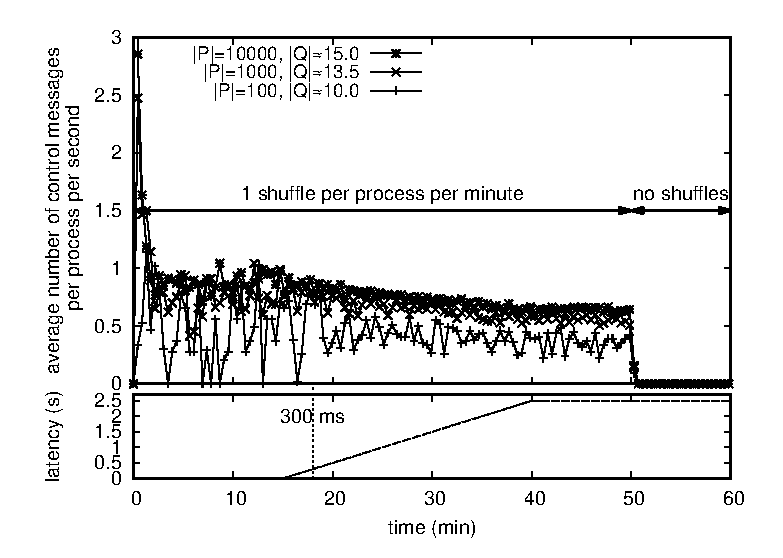
\includegraphics[width=0.65\textwidth]{./img/controlmessages.eps}
%     \caption{\label{fig:controlmessages}Traffic overhead generated by
%       \RPCBROADCAST.  Average number of control messages received --~including
%       routing~-- per process for each second.}
%   \end{center}
% \end{figure*}



%\begin{itemize}[leftmargin=*]
\noindent Figure~\ref{fig:overhead} confirms that the local space consumption
  depends on the in-view size. Systems with larger in-views consume more
  space. Each new delivered message adds control information on each link of the
  in-view (see Algorithm~\ref{algo:reliablebroadcast}).

\noindent Figure~\ref{fig:overhead} confirms that the local space consumption
  depends on network condition. The overhead increases as the latency
  increases. Latency increases the time between the first and the last receipt
  of each message. Processes store messages longer until their safe removal.
  %can be safely removed. 

\noindent Figure~\ref{fig:overhead} confirms that the local space consumption
  depends on broadcast messages. When processes stops broadcasting, the space
  consumed at each process drops to 0. Each process eventually receive each
  message and safely remove the corresponding entry.

\noindent Figure~\ref{fig:overhead} shows that at a rate of 10 broadcasts per second
  and when latency stays under a realistic bound ($300$ milliseconds), the overhead is
  lower than vector-based approaches. Whatever system conditions, it would
  require a vector of 100, 1k entries, 10k entries to forbid multiple delivery
  in the 100-processes system, 1k-processes system, 10k-processes system
  respectively. However, it is worth noting that the overhead of \RPCBROADCAST
  increases linearly with the number of messages currently transiting. 100
  broadcasts per second would multiply measurements made on \RPCBROADCAST by a
  factor of 10. In such case, the 100-entries vector would be better than
  \RPCBROADCAST even under a latency of $300$ milliseconds. 
%\end{itemize}

\noindent \RPCBROADCAST provides a novel trade-off between speed, memory, and
traffic. Among other, its space consumed increases and decreases depending on
the system and its current use; instead of past use (see
Section~\ref{sec:relatedwork}. This result means that it constitutes an
advantageous trade-off in
\begin{inparaenum}[(i)]
\item dynamic systems
\item comprising up to millions of processes
\item that could broadcast at any time.
\end{inparaenum} \\

\noindent \textbf{Objective:} To confirm that the generated traffic overhead
depends on the dynamicity of the system.

\noindent \textbf{Description:} We measure the average number of control
messages received by each process during a second. This includes the routing of
messages. The setup is identical to that of prior experiment.

\noindent \textbf{Results:} Figure~\ref{fig:controlmessages} shows the results of
this experiment. The top part of the figure depicts the traffic overhead
generated by \RPCBROADCAST while the bottom part of the figure depicts the
evolution of transmission delays.

%\begin{itemize}[leftmargin=*]

\noindent Figure~\ref{fig:controlmessages} shows that the number of control messages
  received by processes depends on the dynamicity of the system. The more
  dynamic the higher the traffic overhead. At the beginning of the experiment,
  processes join the system. Numerous links are established at once, hence the
  high number of control messages. Then processes shuffle their out-view during
  50 minutes. The number of links to add and remove is roughly constant over
  time, hence the stabilization in number of control messages. Finally,
  processes stop shuffling at $50$ minutes. Processes do not receive additional
  control messages.

\noindent Figure~\ref{fig:controlmessages} confirms our traffic overhead complexity
  analysis. For instance, in the 10k-processes system, views comprises 15
  processes which belong half from the out-view and half from the in-view.  Each
  process shuffles every minute. Each shuffle adds and removes 7.5 links (twice
  half of the out-view size). Since the peer-sampling protocol establishes links
  using neighbor-to-neighbor interactions, it allows a form of routing where
  only 8 control messages are required to initialize a new link.
  $|exchanged\_links|*|control\_messages|/60 \approx 7.5*8/60 \approx 1$ control
  message per second.

\noindent Figure~\ref{fig:controlmessages} shows that latency smooth and decreases
  the number of control messages. The peer-sampling protocol only shuffles links
  already safe and the memory of which is initialized. Since increasing latency
  increases the initialization time of links, processes exchange less links at
  each shuffle. The generated traffic decreases accordingly. Latency also
  spreads control messages over time, hence the smoothing in measurements.

%\end{itemize}

% Overall, this section empirically confirms that the space complexity of
% \RPCBROADCAST is non-monotonic and depends on the system and its
% usage. Section~\ref{subsec:complexity} states that the space complexity is
% $O(Q_i.M)$ where $Q_i$ is the size of the in-view built by peer-sampling
% protocols, and $M$ is the number of messages that have been delivered but that
% will be received again. This experiment confirms that the space consumed by each
% process increases and decreases over time. In dynamic settings, this comes at
% the cost of control messages to initialize memory link.

\noindent Assuming peer-sampling protocols that enable a form of routing,
\RPCBROADCAST forbids multiple delivery at the cost of a few lightweight control
messages in dynamic systems. In this experiment, the underlying peer-sampling
protocol builds a random graph topology that has numerous desirable properties
such as resilience to failures, or load balancing~\cite{jelasity2007gossip}. It
fits dynamic systems where numerous processes join and leave
continuously. Nonetheless, other peer-sampling protocols could be used depending
on the configuration of the system.
One could minimize latency~\cite{dabek2004vivaldi}, or gather people based on 
user preferences~\cite{jelasity2009tman}.

% One could minimize latency using
% Vivaldi~\cite{dabek2004vivaldi}, or gather people based on user preferences
% using T-Man~\cite{jelasity2009tman}.


% However, it is worth noting that it remains in the hands of developers to choose
% the best peer-sampling protocol for their system (e.g. minimizing
% latency~\cite{dabek2004vivaldi}).


Overall, this section showed that \RPCBROADCAST proposes a novel trade-off in
terms of complexity. Its complexity actually depends on the system (its
dynamicity, its latency, its topology) and current use (broadcasts per second).
\RPCBROADCAST forbids multiple delivery and safely removes obsolete control
information about broadcast messages. The next section reviews state-of-the-art
approaches designed to forbid multiple delivery.




%%% Local Variables:
%%% mode: latex
%%% TeX-master: "../paper"
%%% End:
